\documentclass[usenames,dvipsnames]{beamer}
\usepackage{comment}
\usetheme{CambridgeUS}
%\usepackage{macros_gpi}

%\setbeamertemplate{blocks}[rounded][shadow=false]
\usepackage{epsfig}
\usepackage[french]{babel}
\usepackage[utf8x]{inputenc}
\usepackage[T1]{fontenc}
\usepackage{algorithm}
\usepackage{stmaryrd}
%\usepackage{slashbox}
\usepackage{algorithmic}
\usepackage{multirow}   
\usepackage{pstricks}    
\usepackage{color}   
\usepackage{pifont}
\usepackage{supertabular}   
\usepackage{graphicx}
\usepackage{graphbox}
\usepackage{caption}
\usepackage{subcaption}
\usepackage{animate}
%\usepackage{pdfpc-commands}
%\usepackage{xmpmulti}
\captionsetup[figure]{labelformat=empty}
\usepackage{tikz}
\usetikzlibrary{shadows}
\usepackage{fontawesome}
%\newlength{\myheight}

\usepackage{xcolor}
\definecolor{orange-perp}{rgb}{1.0,0.412,0}
\definecolor{prune-saclay}{rgb}{0.388,0,0.235}
\definecolor{bleu-nice}{rgb}{0,0.686,0.843}
\setbeamercolor{author in head/foot}{bg=black,fg=white}
\setbeamercolor{title in head/foot}{fg=black,bg=white}
\setbeamercolor{frametitle}{fg=black,bg=white}
\setbeamercolor{date in head/foot}{bg=black,fg=white}
\setbeamercolor{section in head/foot}{bg=black,fg=white}
\setbeamercolor{subsection in head/foot}{fg=black,bg=white}
\definecolor{darkspringgreen}{rgb}{0.09, 0.45, 0.27}

\setbeamercolor{block body alerted}{bg=white,fg=gray}
\setbeamercolor{block title alerted}{bg=gray,fg=white}

\setbeamercolor{block body}{bg=black!0.2,fg=black}
\setbeamercolor{block title}{bg=black,fg=white}
%\setbeamercolor{block body}{bg=structure!10}
%\setbeamercolor{block title}{bg=structure!20}

\selectlanguage{french}
\setbeamercolor{footlinecolor}{fg=white,bg=black}
\renewcommand\footnoterule{{\color{black}\hrule height 0.5pt width \paperwidth}}


\usepackage{hyperref}
\hypersetup{
  %colorlinks   = true, %Colours links instead of ugly boxes
  %urlcolor     = blue, %Colour for external hyperlinks
  %linkcolor    = blue, %Colour of internal links
  %citecolor   = red %Colour of citations
}

%\setbeamercolor{itemize item}{fg=prune}
%\setbeamercolor{itemize subitem}{fg=prune}
%\setbeamercolor{itemize subsubitem}{fg=prune}

%\setbeamertemplate{itemize item}[ball]{fg=prune}
%\setbeamertemplate{itemize subitem}[ball]{fg=prune}
%\setbeamertemplate{itemize subsubitem}[triangle]


\setbeamertemplate{itemize item}{%
    \begin{tikzpicture}
        \shade[ball color=black!100!white] (0,0) circle (0.6ex);
    \end{tikzpicture}
}

\setbeamertemplate{itemize subitem}{%
    \begin{tikzpicture}
        \shade[ball color=black!100!white] (0,0) circle (0.6ex);
    \end{tikzpicture}
}


\setbeamercolor*{title}{use=structure,fg=white,bg=black!95}
\setbeamertemplate{title page}[default][colsep=-4bp,rounded=true,shadow=true]
\setbeamertemplate{navigation symbols}{} 
%\setbeamerfont{section number projected}{size=\footnotesize}
%\setbeamercolor{section number projected}{bg=prune,fg=white}
%\setbeamercolor{section in toc}{fg=prune}
%\setbeamercolor{subsection in toc}{fg=prune}
%\setbeamercolor{subsection number projected}{bg=prune}

\setbeamercolor{section number projected}{bg=black,fg=white}
\setbeamercolor{section in toc}{fg=black}
\setbeamercolor{subsection in toc}{fg=black}
\setbeamercolor{subsection number projected}{bg=black}

%\setbeamertemplate{subsections in toc}[square]
\mode<all>

%\setbeamertemplate{footline}{
%\begin{picture}(0,0)(0,0)
%\put(320,4){\footnotesize \insertframenumber{}/\inserttotalframenumber{}}
%\end{picture}
%}
\usepackage{hyperref}
\usepackage{siunitx}

\graphicspath{{fig/}}

%\includegraphics[width=1cm]{logo-projet-finance-par-ANR.jpg}
\title[\textbf{Dark-era project}]{\textbf{Dark-era - Session\#1}} 
\subtitle{Dataflow Algorithm aRchitecture co-design of SKA pipeline for Exascale Radio Astronomy\\ }
\institute[]{Daniel Charlet$^{**5}$ (IJCLab), Karol Desnos$^{1}$, Mickael Dardaillon$^{3}$, André Ferrari$^{4}$, Chiara Ferrari$^{4}$, \underline{Nicolas Gac$^{3}$}, Jean-François Nezan$^{1}$, François Orieux$^{3}$, Simon Prunet$^{4}$, Martin Quinson$^{2}$, Frédéric Suter$^{**2}$(IN2P3 Computing Center), Cyril Tasse$^{**5}$ (GEPI), Cédric Viou$^{5}$ }
\author[IETR/IRISA/L2S/Lagrange/Nançay]{$^{1}$IETR (INSA),  $^{2}$IRISA (ENS), $^{3}$L2S (CS), $^{4}$Lagrange (UCA),  $^{5}$Nançay (Obs Paris)}
\date{ISC 2021 - project session}


\newcommand{\mysection}[2][blue]{%
    \begingroup
    \setbeamercolor{background canvas}{bg=#1}
    \setbeamercolor{section title}{fg=-#1}
    \section{#2}
    \endgroup
}

\begin{document}

%\frame[plain]{\titlepage}

{
\usebackgroundtemplate{\tikz\node[opacity=0.7]
  {
    \hspace{-0.25cm} 
\includegraphics[width=\paperwidth]{ISC2021_Title-Slide}};
}

\frame[plain]{
   %\titlepage
   \vspace{4.5cm}
   \begin{columns}[t]
    \begin{column}{.45\linewidth}
    \end{column}
    \begin{column}{.55\linewidth}
        \begin{columns}[t]
            \begin{column}{.4\linewidth}
                \begin{center}
        \includegraphics[width=0.9\textwidth]{DARKERA_logo_color.pdf}  
    \end{center}
    \end{column}
    \begin{column}{.6\linewidth}
        \begin{center}
         %\begin{minipage}{\linewidth}
            \begin{center}
            \large{\textbf{Dark-Era Project}}
\vspace{0.5cm}
            \scriptsize{Poster Session \\ June 30 2021}
        \end{center}
         %\end{minipage}
            
         \end{center}
    \end{column}
\end{columns}
    \end{column}
    \end{columns}

    \vspace{0.1cm}

    \begin{columns}[t]
        \begin{column}{.85\linewidth}
   \begin{center}
   \tiny{
\begin{minipage}{\linewidth}
   Daniel Charlet$^{**5}$ (IJCLab), Karol Desnos$^{1}$, Mickael Dardaillon$^{3}$, André Ferrari$^{4}$, Chiara Ferrari$^{4}$, \underline{Nicolas Gac$^{3}$}, Jean-François Nezan$^{1}$, François Orieux$^{3}$, Simon Prunet$^{4}$, Martin Quinson$^{2}$, Frédéric Suter$^{**2}$(IN2P3 Computing Center), Cyril Tasse$^{**5}$ (GEPI), Cédric Viou$^{5}$\\
   \\
   $^{1}$IETR (INSA),  $^{2}$IRISA (ENS), $^{3}$L2S (CS), $^{4}$Lagrange (UCA),  $^{5}$Nançay (Obs Paris) 
\end{minipage}
   }
\end{center}
\end{column}
\begin{column}{.15\linewidth}
    \begin{center}
        %\scalebox{0.2}{ \input{logo_ANR_avec_numero_projet.pdf_t}}
        
\includegraphics[width=0.75\textwidth]{anr-light.pdf}    \\ 
        \tiny{ \scalebox{0.75}{ANR-20-CE46-0001-01}}
    \end{center}
    \end{column}
\end{columns}
}
}
\frame[noframenumbering]{\tableofcontents}

\section{SKA context}
\subsection{SKA computing, an HPC challenge}

\frame{
\scriptsize{
\begin{columns}[t]
    \begin{column}{.4\linewidth}
\begin{center}
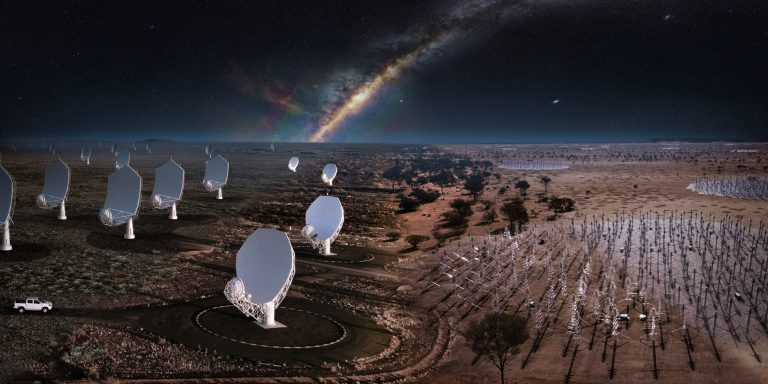
\includegraphics[width=\textwidth]{SKA-at-Night-768x384.jpg} 
\end{center}
\end{column}
\begin{column}{.6\linewidth}
    \begin{block}{SKA}
        aa
    \end{block}
\end{column}
\end{columns}

\begin{columns}[t]
    \begin{column}{.4\linewidth}
\begin{center}
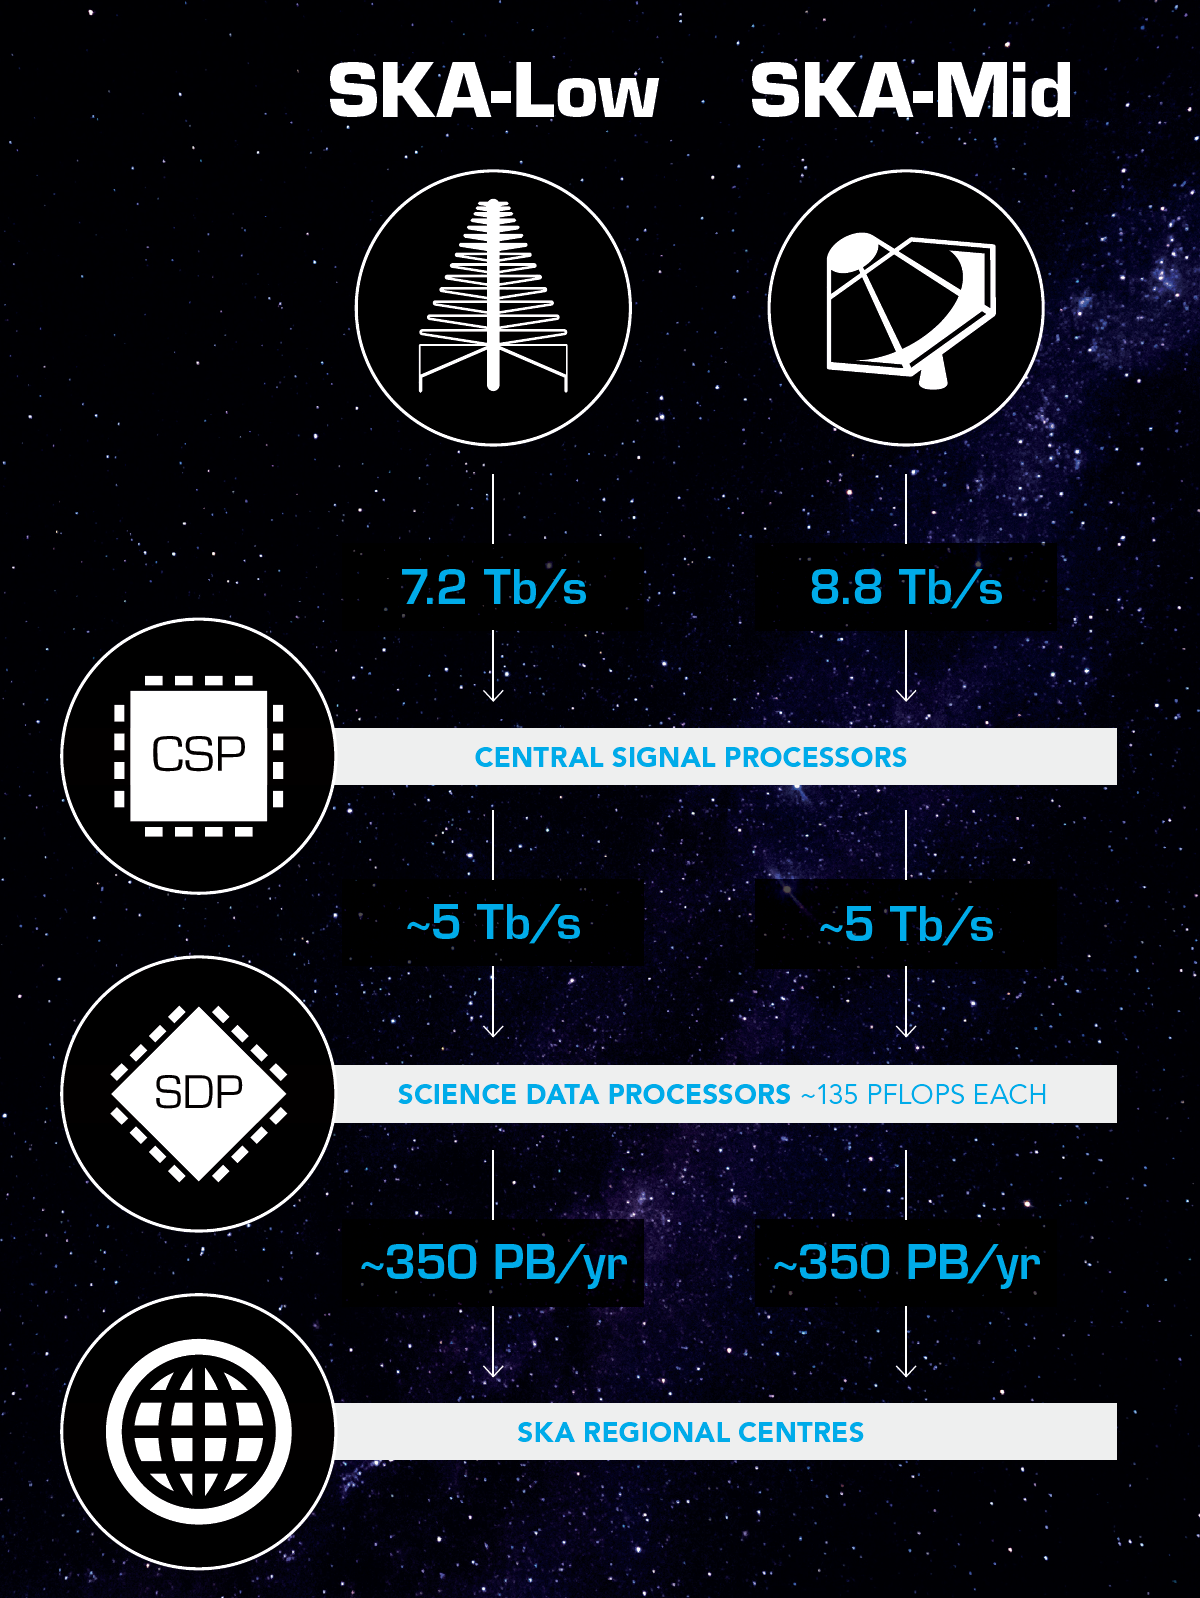
\includegraphics[width=0.7\textwidth]{image002}
\end{center}
\end{column}
\begin{column}{.6\linewidth}
    \begin{block}{SDP}
        aa
    \end{block}
\end{column}
\end{columns}
}
}


\section{Team}
\subsection{Interdisciplinarity}


\frame{
    \centering
    %\frametitle{An interdisciplinary Team}
    \includegraphics[width=\textwidth]{team_DARK-ERA.pdf}  
    
}

\subsection{Open Positions}
\frame{
    \centering
    %\frametitle{Open positions}
    \scriptsize{
    \begin{block}{Post-doc at LS2}
        \begin{itemize}
            \item \underline{Title}: \textit{Radioastronomy imager accelerated on FPGA through High Level Synthesis}
            \item \underline{Application}: as soon as possible
            \item \href{https://l2s.centralesupelec.fr/job/dark-era-postdoc/}{\textcolor{blue}{https://l2s.centralesupelec.fr/job/dark-era-postdoc/}}
           % \item \textcolor{gray}{Post-doc at Lagrange on algorithm/architecture exploration for radioastronomy (spring 2024)}
        \end{itemize}
    \end{block}

    \begin{block}{Internship/PhD at IETR}
        \begin{itemize}
            \item \underline{Title}: \textit{Design and Programming of Low-Power High Performance Computing Systems in Astronomy} 
            \item \underline{Application}: as soon as possible
            \item \href{https://codimd.math.cnrs.fr/OXqnp\_JiRPGc56ghEWHP2w}{\textcolor{blue}{https://codimd.math.cnrs.fr/OXqnp\_JiRPGc56ghEWHP2w}}
        \end{itemize}
    \end{block}

    \begin{block}{Internship/PhD at IRISA}
        \begin{itemize}
            \item \underline{Title}: \textit{Workflow vs. Dataflow: Concepts, challenges and simulation for high performance computing} 
            \item \underline{Application}: as soon as possible
            \item \href{https://cclab.pages.in2p3.fr/web/downloads/dark-era\_xflow.pdf}{\textcolor{blue}{https://cclab.pages.in2p3.fr/web/downloads/dark-era\_xflow.pdf}}
        \end{itemize}
    \end{block}

    \begin{alertblock}{Posdoc at Lagrange (2023)}
        \begin{itemize}
            \item \underline{Title}: \textit{Algorithm and Architecture exploration for radioastronomy imager} 
        \end{itemize}
    \end{alertblock}

    }
    
}


\setbeamercolor{background canvas}{bg=black}
\section*{End}
\frame[t,noframenumbering]
{
  
%\frametitle{Projet ANR DARK-ERA (2/2)}
\vspace{2.6cm}
\centering
{\huge\textcolor{white}{Thank you for your attention !}\\
\vspace{1cm}
\href{https://dark-era.pages.centralesupelec.fr}{\textcolor{white}{https://dark-era.pages.centralesupelec.fr}}
}

}

\end{document}

